\titre{}
\theme{calcLit}
\auteur{Nathan Scheinmann}
\niveau{1M}
\source{musy}
\type{serie}
\piments{2}
\pts{}
\annee{2425}

\contenu{
\tcblower
En Grèce antique on donnait des preuves géométriques des propriétés des nombres réels, basées sur l'aire du rectangle. 
	\begingroup
{%% do not forget to chage the default values inside a group
\belowdisplayskip=-10pt
	\begin{tasks}
	\task 	Pour illustrer la distributivité de la multiplication sur l'addition pour les nombres réels $a,b,$ et $c$, exprimer de deux manières l'aire du rectangle représenté ci-dessous\,:

	\begin{center}
	
\begin{tikzpicture}
    \tkzDefPoint[label=below:{}](-1,-1){A}
    \tkzDefPoint[label=right:{}](-1,1){B}
    \tkzDefPoint[label=above:{}](2,1){C}
    \tkzDefPoint[label=above:{}](2,-1){D}
    \tkzDefPoint[label=above:{}](3,1){E}
    \tkzDefPoint[label=above:{}](3,-1){F}

    \tkzDrawPolygon(A,B,E,F)
    \tkzDrawSegment[dashed,dim={$b$,15pt,midway,font=\footnotesize}](B,C)
    \tkzDrawSegment[dashed,dim={$c$,15pt,midway,font=\footnotesize}](C,E)
    \tkzDrawSegment[dashed,dim={$a$,15pt,midway,font=\footnotesize}](A,B)
    \tkzDrawSegment[dashed](C,D)
	\end{tikzpicture}
\end{center}
	\task De manière semblables, illustrer géométriquement les identités suivantes puis les prouver\;:
	\[(a+b)^2 \quad \text{et}\quad (a+b)(c+d)\]
	\end{tasks}
}\endgroup
}
\correction{
\tcblower
\begin{tasks}
	\task $ab+ac$ ou $a(b+c)$, d'où la distributivité simple. 
	\task 
	
	\begin{minipage}[t]{0.45\textwidth}{
	\vspace{0pt}
		\begin{center}
	\begin{tikzpicture}
    \tkzDefPoint[label=below:{}](-1,-1){A}
    \tkzDefPoint[label=right:{}](-1,3){B}
    \tkzDefPoint[label=above:{}](2,3){C}
    \tkzDefPoint[label=above:{}](2,-1){D}
    \tkzDefPoint[label=above:{}](3,3){E}
    \tkzDefPoint[label=above:{}](3,-1){F}
    \tkzDefPoint[label=above:{}](-1,2){G}
    \tkzDefPoint[label=above:{}](3,2){H}

    \tkzDrawPolygon(A,B,E,F)
    \tkzDrawSegment[dashed,dim={$a$,15pt,midway,font=\footnotesize}](B,C)
    \tkzDrawSegment[dashed,dim={$b$,15pt,midway,font=\footnotesize}](C,E)
    \tkzDrawSegment[dashed,dim={$a$,15pt,midway,font=\footnotesize}](A,G)
    \tkzDrawSegment[dashed,dim={$b$,15pt,midway,font=\footnotesize}](G,B)
    \tkzDrawSegment[dashed](C,D)
    \tkzDrawSegment[dashed](G,H)
	\end{tikzpicture}
\end{center}
	}
	\end{minipage}
	\begin{minipage}[t]{0.45\textwidth}{
	\vspace{0pt}
		\begin{center}
	\begin{tikzpicture}
    \tkzDefPoint[label=below:{}](-1,-1){A}
    \tkzDefPoint[label=right:{}](-1,1){B}
    \tkzDefPoint[label=above:{}](2,1){C}
    \tkzDefPoint[label=above:{}](2,-1){D}
    \tkzDefPoint[label=above:{}](3,1){E}
    \tkzDefPoint[label=above:{}](3,-1){F}
    \tkzDefPoint[label=above:{}](-1,-0.3){G}
    \tkzDefPoint[label=above:{}](3,-0.3){H}

    \tkzDrawPolygon(A,B,E,F)
    \tkzDrawSegment[dashed,dim={$c$,15pt,midway,font=\footnotesize}](B,C)
    \tkzDrawSegment[dashed,dim={$d$,15pt,midway,font=\footnotesize}](C,E)
    \tkzDrawSegment[dashed,dim={$a$,15pt,midway,font=\footnotesize}](A,G)
    \tkzDrawSegment[dashed,dim={$b$,15pt,midway,font=\footnotesize}](G,B)
    \tkzDrawSegment[dashed](C,D)
    \tkzDrawSegment[dashed](G,H)
	\end{tikzpicture}
\end{center}
	}
	\end{minipage}

	Écrire l'aire de deux manière à chaque fois pour prouver les identités.
\end{tasks}
}
